\subsection{Controllers}
Assim que um pedido consegue ultrapassar todos os \textit{middlewares} sem ser impedido, este é redirecionado para um \textit{controller}.

\subsubsection{Estruturação dos controllers}
Para evitar a variação de código destes \textit{controllers} em termos de estrutura, foi decidido desenhar uma estrutura de \textit{controller} e aplicar perante o demais código. Esta segue as seguintes etapas:
\begin{enumerate}
 \item Obter dados do pedido
 \item Validar se os dados obrigatórios são obtidos
 \item Validar o pedido perante o modelo de negócio
 \item Executar a lógica do pedido
 \item Formular a resposta e enviar
 \item Em caso de erro este deverá ser capturado e processado para enviar um erro para o utilizador
\end{enumerate}

 Esta estrutura será sempre aplicada, pois, foram utilizados \textit{snippets} de código que permitem criar um modelo de estrutura, apenas é necessário escrever a palavra-chave e toda a estrutura é aplicada, pelo que, é necessário de seguida efetuar as alterações perante o contexto.

\subsubsection{Execução da lógica de negócio}
A execução da lógica de negócio passa por direcionar os dados para a ação correta. Esta ação geralmente resulta numa operação de base de dados. Inicialmente foi desenvolvida toda a validação de código e todas as operações de base de dados diretamente na execução da lógica de negócio. Após uma revisão desta organização de código com o professor orientador, foi decidido separar estas funcionalidades. Daqui surgiu a componente de validação de dados, a de operações de base de dados e a de lógica de negócio, que implementa a componente de operações de base de dados. Sendo assim, para evitar que estas operações sobre a base de dados estejam em conjunto com o direcionamento dos dados, foram criados modelos para cada tabela. Cada modelo contém um conjunto de operações sobre a tabela correspondente. Estas operações, estão contidas sobre métodos que podem receber dados para executar na operação e devolver a resposta da mesma.

\newpage

\subsubsection{Validação dos dados}
A validação dos dados é necessária para evitar erros a nível de servidor com dados em falta e também para aplicar as regras de negócio. Para realizar estas validações, é necessário em primeiro lugar verificar se todos os dados são recebidos, de seguida, são enviados para um \textit{validator}. O \textit{validator} executa todas as verificações necessárias a nível de regras de negócio, na possibilidade de alguma regra não ser cumprida, é atirado um erro.

\subsubsection{Formulação da resposta}
Como mencionado no capítulo \ref{sec:idioma_comunicacao}, o bem mais importante numa boa comunicação é a utilização da mesma linguagem, pelo que, a resposta do servidor deverá utilizar a linguagem indicada pelo utilizador. Para realizar esta tradução foi utilizado o mesmo conceito que se usa em \textit{Android}. Neste é desenvolvido um ficheiro que contém um conjunto de chaves e a cada corresponde um texto. Cada tradução tem de conter estas chaves para que seja possível obter o texto correto para cada uma. Sendo assim, foi utilizado um ficheiro \textit{\acrshort{json}} que dispõem das chaves das linguagens suportadas. A cada uma corresponde a um conjunto de outras chaves que com todas as traduções necessárias. Esta abordagem permite que de forma fácil, futuramente seja possível adicionar outras linguagens ao servidor.

\begin{figure}[htb]%
 \centering
 \subfloat[\centering Página de login]{{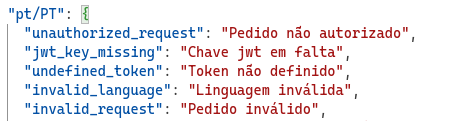
\includegraphics[width=0.45\textwidth]{images/implementacao/api/trad_pt.png} }}%
 \qquad
 \subfloat[\centering Página de registo]{{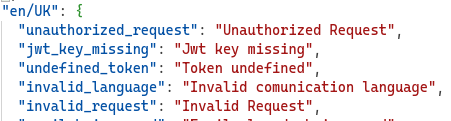
\includegraphics[width=0.45\textwidth]{images/implementacao/api/trad_en.png} }}%
 \caption{Autenticação - Login e Registo}%
 \label{fig:24}
\end{figure}

O suporte a este ficheiro foi elaborado com uma operação que recebe a chave e a linguagem desejada. Este devolve o texto traduzido, dado que, na formulação da resposta a operação é executada com a indicação da chave do texto a enviar e a linguagem desejada, sendo que este é devolvido para o utilizador.

\subsubsection{Processamento de erros}
Como não é de interesse enviar erros do próprio servidor para o utilizador, foi decidido controla-los. Para isso foi concebido um erro customizado com base no erro da própria linguagem. Este recebe por parâmetro o código da tradução da mensagem. Esta abordagem permite evitar que sempre que um erro é lançado o sistema pare. Contudo, sempre que um erro é lançado pela base de dados, erro de código ou de biblioteca, o original é chamado, o que levou a que sempre que é detetado é devolvida uma mensagem de "erro de servidor", isto evita a que dados sensíveis e desnecessários para o utilizador sejam devolvidos.